\documentclass[11pt,a4paper]{article}
\usepackage[margin=22mm]{geometry}
\usepackage[T1]{fontenc}
\usepackage{lmodern}
\usepackage{tabularx,booktabs,hyperref,xcolor,array,xurl}
\usepackage{tikz}
\usetikzlibrary{arrows.meta,positioning,fit,shapes.geometric}
\usepackage{enumitem}
\usepackage{listings}
\hypersetup{colorlinks=true,linkcolor=blue,urlcolor=blue,citecolor=blue}
\setlength{\parindent}{0pt}\sloppy
\setlength{\parskip}{6pt}
\renewcommand{\arraystretch}{1.15}
\newcolumntype{Y}{>{\raggedright\arraybackslash}X}
\newcolumntype{P}[1]{>{\raggedright\arraybackslash}p{#1}}
\newcommand{\code}[1]{\nolinkurl{#1}}
\newcommand{\status}[1]{\textbf{#1}}
\title{}
\author{}
\date{}

\begin{document}
\begin{center}
{\Large\textbf{23CSE455 Design Patterns}}\\[4pt]
{\LARGE\textbf{Case Study Report}}\\[6pt]
{\large Design Pattern Identification and Evolution in a Spring MVC-Based Warehouse Management Application}
\end{center}

\textbf{Team: B9}\\
\textbf{Date: 10 October 2026} (findings re-audited 11 October 2026)\\
\textbf{Submission repository:} \href{https://github.com/aswathymohan-amrita/23CSE455_DP_CaseStudy}{23CSE455\_DP\_CaseStudy}\\
\textbf{Team working repository:} \href{https://github.com/akdswordguy/Team_B9_DP}{akdswordguy/Team\_B9\_DP}


\begin{tabularx}{\linewidth}{@{}P{0.25\linewidth}P{0.19\linewidth}P{0.10\linewidth}X@{}}
\toprule
Roll number & Student name & Batch \\
\midrule
AM.SC.U4CSE23215 & D Aditya Kiran & CSE C \\
AM.SC.U4CSE23235 & Mithun Krishna & CSE C \\
AM.SC.U4CSE23248 & Sai Kishen K M & CSE C\\
AM.SC.U4CSE23359 & Sivadev Smijith & CSE D \\
\bottomrule
\end{tabularx}

Per-part findings documents with full evidence tables accompany this report: \code{report/part1_findings.pdf}, \code{report/part2_findings.pdf}, and \code{report/part3_findings.pdf}. Unless stated otherwise, evidence paths below are relative to \code{Team_B9_Findings/} in the team working repository.

\section{Application and architecture}

\subsection{Original source and baseline}
The application studied is OpenWMS, an open-source warehouse-management system built from Java/Spring Boot components. OpenWMS is split across several repositories; three were inspected, each at an exact baseline commit:

\begin{tabularx}{\linewidth}{@{}P{0.36\linewidth}YP{0.30\linewidth}@{}}
\toprule
Repository & Role in this study & Baseline commit\\
\midrule
\href{https://github.com/openwms/org.openwms}{\nolinkurl{openwms/org.openwms}} (CORE) & Part 1 pattern inspection; contains the \code{org.openwms.core.util} library & \code{9d263bf65ec75301e0302539ae7bf581412742b8}\\
\href{https://github.com/openwms/org.openwms.common.service.lib}{\nolinkurl{openwms/org.openwms.common.service.lib}} & Multiple-Warehouse Support (Part 2) & \code{a6566d7a90364f8cb0e82ec013720b644926dffe}\\
\href{https://github.com/openwms/org.openwms.common.service}{\nolinkurl{openwms/org.openwms.common.service}} & Multiple-Warehouse Support (Part 2) & \code{fc7edd4ffbe16de65d482b3a2d462d4d896b1998}\\
\bottomrule
\end{tabularx}

The CORE repository was clean at inspection. \textbf{Multiple-Warehouse Support} changes in the two Common Service worktrees were not committed at the time of the recorded audit.

OpenWMS repositories inspected in this work are distributed under the Apache License 2.0. Their copyright, licence, provenance, and exact baseline commits must be preserved when republishing patches or source excerpts. The \textbf{Barcode-Based Picking} and \textbf{Automatic Stock Reordering} projects and the Part 3 implementations are separate case-study reference projects, not modifications to the canonical Picking and Inventory modules, which were inaccessible (Section~1.3).

\subsection{Environment}
The inspected application and evolution projects use Java and Maven. \textbf{Barcode-Based Picking} and \textbf{Automatic Stock Reordering} verification was performed with Maven and Java in the local Windows environment. Part 3 toolchains recorded in \code{PART3_EVIDENCE.md} were OpenJDK 25.0.4.1, Python 3.13.15, Node.js 24.21.0, and g++ 16.2.0; the 11 October re-audit re-ran Part 3 with OpenJDK 21.0.12.1, Python 3.13.16, Node.js 22.22.0, and g++ 13.3.0. Static complexity was measured with Lizard 1.24.1. Exact dependency versions for each upstream module should be taken from its checked-in Maven descriptors and are not inferred here.

\subsection{Scope and exclusions}
Part 1 examined the \code{org.openwms.core.util} module of the CORE repository (64 Java files at the baseline) for two candidate GoF collaborations: the event-dispatching collaboration involving \code{EventBroker}, \code{EventDispatcher}, \code{EventListener}, \code{SimpleEventDispatcher}, and \code{RootApplicationEvent}; and the generic tree utility \code{TreeNode<T>} / \code{TreeNodeImpl<T>}. Three further non-GoF mechanisms were recorded separately (Section~2.6). Candidate patterns were accepted only where source relationships and behavior supported the pattern interpretation. Singleton and Proxy were assessed and rejected. The repository contains no concrete client of the generic Composite utility and no concrete implementation of \code{EventListener}; both limitations are retained in the findings.

\textbf{Multiple-Warehouse Support} modifies the Common Service Library and Common Service worktrees to model multiple warehouses. \textbf{Barcode-Based Picking} and \textbf{Automatic Stock Reordering} are isolated reference implementations because the canonical modules could not be modified: the CORE README lists the Picking Library as a private, GPLv3-licensed repository and the Inventory Service as private preview. Part 3 contains small independent implementations of Observer and Composite in four languages; they are not claimed to be OpenWMS production code.

\subsection{Architecture and request/event flow}
OpenWMS uses a microservice architecture in which each business component is a Spring Boot service in its own repository. The CORE repository is not itself a service: its README states that it holds project-level documentation and one Maven module, \code{org.openwms.core.util}, a library of utilities, exception types, and shared event types. The Spring MVC controllers and service logic referred to in the title live in the service repositories such as Common Service. The diagram below is a scope diagram, not a claim that every shown module is deployed in one process or that the Composite utility is used by a specific business workflow.

\begin{center}
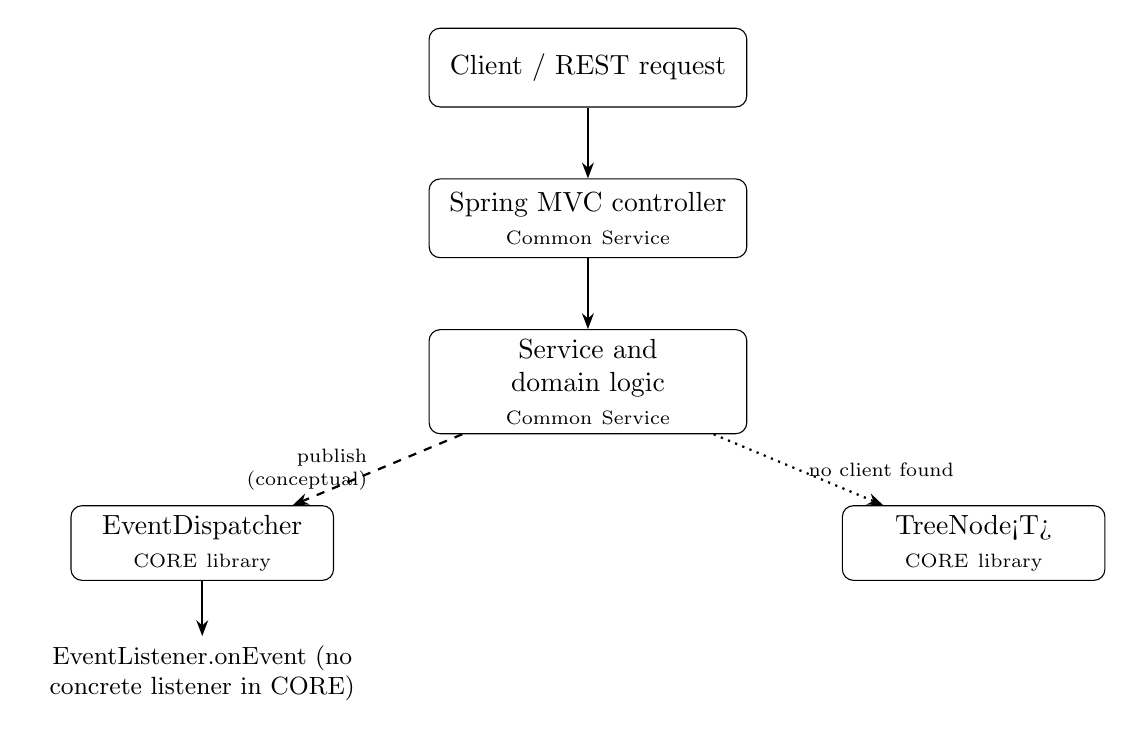
\begin{tikzpicture}[
  node distance=9mm and 12mm,
  box/.style={draw,rounded corners,align=center,text width=38mm,minimum height=10mm},
  smallbox/.style={draw,rounded corners,align=center,text width=31mm,minimum height=9mm},
  arr/.style={-{Stealth[length=2mm]},thick}
]
\node[box] (client) {Client / REST request};
\node[box,below=of client] (mvc) {Spring MVC controller\\\scriptsize Common Service};
\node[box,below=of mvc] (service) {Service and domain logic\\\scriptsize Common Service};
\node[smallbox,below left=of service] (event) {\code{EventDispatcher}\\\scriptsize CORE library};
\node[smallbox,below right=of service] (tree) {\code{TreeNode<T>}\\\scriptsize CORE library};
\draw[arr] (client)--(mvc);
\draw[arr] (mvc)--(service);
\draw[arr,dashed] (service)--node[left,font=\scriptsize,align=right]{publish\\(conceptual)}(event);
\draw[arr,dotted] (service)--node[right,font=\scriptsize]{no client found}(tree);
\node[below=7mm of event,align=center,text width=42mm,font=\small] (listener) {\code{EventListener.onEvent} (no concrete listener in CORE)};
\draw[arr] (event)--(listener);
\end{tikzpicture}
\end{center}

\textbf{Event flow.} A producer calls \code{EventPublisher.publish}; \code{NonBlockingEventPublisherImpl} forwards the event asynchronously (Spring \code{@Async}) to \code{EventDispatcher.dispatch}, and \code{SimpleEventDispatcher} synchronously calls \code{onEvent} on each \code{EventListener} subscribed to that event's exact class. No concrete producer or listener call was traced in the inspected source. The generic tree utility supports parent/child composition and navigation, but no warehouse business workflow in the inspected source uses it.

\subsection{Run instructions and recorded results}
For the upstream modules, use the module README and Maven descriptors for setup. \textbf{Multiple-Warehouse Support} verification was recorded against the existing Common Service Library and Common Service worktrees; the exact baseline and verification addendum are in \code{LLM_RECORDS/LLM_RECORDS.md}. \textbf{Barcode-Based Picking} and \textbf{Automatic Stock Reordering} can be run independently from their project roots with Maven:
\begin{itemize}[nosep]
\item \textbf{Barcode-Based Picking}: \code{mvn.cmd -DforkCount=0 verify} --- recorded \texttt{BUILD SUCCESS}, 14/14 tests.
\item \textbf{Automatic Stock Reordering}: \code{mvn.cmd -DforkCount=0 verify} --- recorded \texttt{BUILD SUCCESS}, 19/19 tests.
\end{itemize}
The \code{-DforkCount=0} option runs tests in the Maven process and may affect test isolation compared with forked execution. Maven could not be re-run during the re-audit because Maven Central was blocked in the audit environment, so these totals are the team's recorded runs; the source-level test counts were re-checked and match. For Part 3, use the per-language commands documented in \code{Part3-cross-language/PART3_EVIDENCE.md}; all eight implementations passed their recorded harness checks and passed again in the re-audit. The original project does not have a single verified, reproducible one-command build documented by this case study.

\section{Part 1 Pattern discovery}

\subsection{Method}
Candidates were assessed through source-level role and relationship mapping, not by names alone. For each candidate, the inspection considered intent, collaborating types, method signatures and bodies (registration, notification, delegation, child management), and available behavior. Every line citation was re-checked against the upstream baseline in the re-audit and found exact, and the copied files under \code{Part1_Findings/evidence/source/} are byte-identical to upstream. The evidence bundle is \code{Part1_Findings/Part1_Findings.md}, \code{Part1_Findings/data/patterns.csv}, \code{Part1_Findings/data/rejected_candidates.csv}, \code{Part1_Findings/data/pattern_counts.csv}, \code{Part1_Findings/evidence/verification_notes.md}, and the PlantUML sources with rendered PNGs in \code{Part1_Findings/diagrams/}.

\subsection{Totals at the baseline}
\begin{tabularx}{\linewidth}{@{}l r Y@{}}
\toprule
Measure & Count & Interpretation\\
\midrule
Confirmed GoF pattern types & 2 & Observer and Composite.\\
Confirmed pattern instances & 2 & One event-dispatching Observer collaboration and one generic tree Composite collaboration.\\
Concrete participant classes & 2 & \code{SimpleEventDispatcher} and \code{TreeNodeImpl<T>}.\\
Unique participant symbols & 7 & Five in the Observer mapping and two in the Composite mapping; no symbol is shared.\\
Rejected candidates assessed & 2 & Singleton and Proxy were assessed and rejected for insufficient supporting evidence.\\
Uncertain candidates & 0 recorded & No separate uncertain candidate is counted in the frozen inventory; this does not mean all possible patterns in the whole product were exhaustively ruled out.\\
\bottomrule
\end{tabularx}

The scope is the accessible source examined, not a claim that the entire OpenWMS ecosystem contains only two design patterns.

\subsection{Pattern inventory}
\begin{tabularx}{\linewidth}{@{}lYrr@{}}
\toprule
Pattern type & Instance name & Instances & Concrete classes\\
\midrule
Observer & OpenWMS event subscription and dispatch & 1 & 1\\
Composite & Generic \code{TreeNode} hierarchy & 1 & 1\\
\bottomrule
\end{tabularx}

\subsection{Instance 1: OpenWMS event subscription and dispatch}
\textbf{Pattern and category.} Observer --- GoF behavioral pattern.

\textbf{Purpose and origin.} The collaboration decouples code that raises application events from the listeners that react to them, through explicit subscription, unsubscription, and dispatch. It is part of the inspected OpenWMS source, rather than a pattern introduced by this case study.

\textbf{Participant mapping} (paths relative to \code{org.openwms.core.util/src/main/java/org/openwms/core/})\par\smallskip
\noindent\begin{tabular}{@{}P{0.22\linewidth}P{0.25\linewidth}P{0.45\linewidth}@{}}
\toprule
Pattern role & Actual symbol & Evidence location\\
\midrule
Subject: attach/detach & \code{EventBroker} & \code{event/EventBroker.java:19-56}; \code{subscribe}/\code{unsubscribe} by listener or bean name.\\
Subject: notify & \code{EventDispatcher} & \code{event/EventDispatcher.java:19-34}; extends \code{EventBroker}, adds \code{dispatch}.\\
ConcreteSubject & \code{SimpleEventDispatcher} & \code{event/SimpleEventDispatcher.java:27-38, 54-56, 75-79, 99-106}.\\
Observer & \code{EventListener} & \code{event/EventListener.java:19-31}; \code{onEvent(RootApplicationEvent)}.\\
Event payload & \code{RootApplicationEvent} & \code{event/RootApplicationEvent.java:23-29}; extends Spring \code{ApplicationEvent}.\\
ConcreteObserver & --- & None: no class in the repository implements \code{EventListener}.\\
\bottomrule
\end{tabular}

\textbf{Evidence and verification.} The defining Observer behavior is present: listeners attach and detach at runtime, and \code{dispatch} iterates the registered set and invokes the common update method \code{onEvent}; the subject never refers to a concrete listener type. The subject role is split across two interfaces and one class rather than invented as a single \code{Subject} type. \code{NonBlockingEventPublisherImpl} calls \code{dispatch} asynchronously; in GoF terms it is a client that triggers notification, so it is recorded as the separate mechanism N01 rather than counted as a participant. The diagram below is a conceptual role diagram; \code{Part1_Findings/diagrams/observer_uml.puml} is the editable source.

\begin{center}
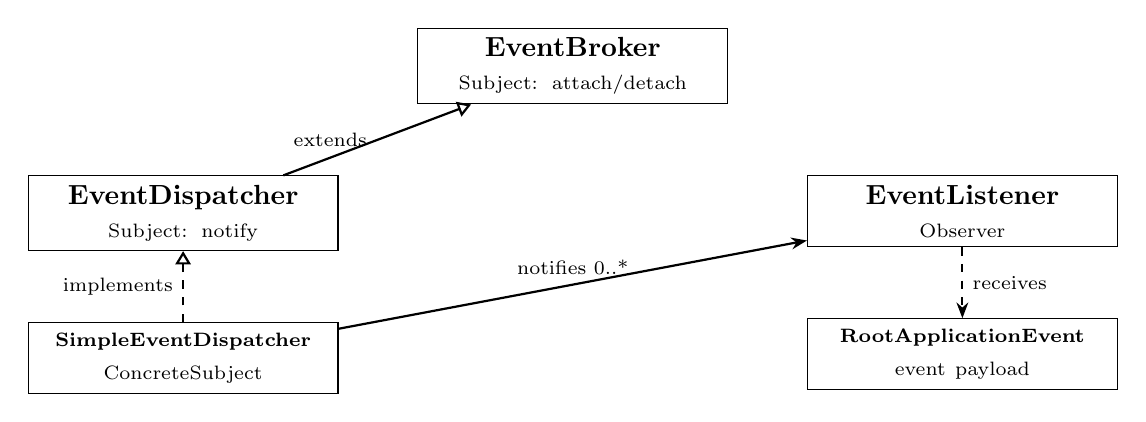
\begin{tikzpicture}[
  node distance=9mm and 10mm,
  cls/.style={draw,align=center,text width=37mm,minimum height=9mm},
  arr/.style={-{Stealth[length=2mm]},thick}
]
\node[cls] (broker) {\textbf{EventBroker}\\\scriptsize Subject: attach/detach};
\node[cls,below left=of broker] (dispatcher) {\textbf{EventDispatcher}\\\scriptsize Subject: notify};
\node[cls,below right=of broker] (listener) {\textbf{EventListener}\\\scriptsize Observer};
\node[cls,below=of dispatcher] (simple) {\textbf{\scriptsize SimpleEventDispatcher}\\\scriptsize ConcreteSubject};
\node[cls,below=of listener] (event) {\textbf{\scriptsize RootApplicationEvent}\\\scriptsize event payload};
\draw[arr,-{Triangle[open]}] (dispatcher)--node[left,font=\scriptsize]{extends}(broker);
\draw[arr,dashed,-{Triangle[open]}] (simple)--node[left,font=\scriptsize]{implements}(dispatcher);
\draw[arr] (simple)--node[above,font=\scriptsize]{notifies 0..*}(listener);
\draw[arr,dashed] (listener)--node[right,font=\scriptsize]{receives}(event);
\end{tikzpicture}
\end{center}
\textbf{Observations and limitations.} (i) \code{dispatch} looks up listeners by \code{event.getClass()}, so a listener subscribed to \code{RootApplicationEvent} is not notified of a subclass event such as \code{UserChangedEvent}. (ii) \code{SimpleEventDispatcher} notifies subscribers sequentially and synchronously. (iii) With no ConcreteObserver in scope, the instance is confirmed at library level.

\subsection{Instance 2: Generic tree hierarchy}
\textbf{Pattern and category.} Composite --- GoF structural pattern (transparent variant, single implementation class).

\textbf{Purpose and origin.} \code{TreeNode<T>} defines a node holding a data value and an identifier-keyed collection of child nodes of the same type, so hierarchies of any depth can be built and navigated through one abstraction. It is a utility-level collaboration present in OpenWMS source.

\textbf{Participant mapping}\par\smallskip
\noindent\begin{tabular}{@{}P{0.22\linewidth}P{0.25\linewidth}P{0.45\linewidth}@{}}
\toprule
Pattern role & Actual symbol & Evidence location\\
\midrule
Component & \code{TreeNode<T>} & \code{util/TreeNode.java:23-115}; data, \code{isLeaf}, \code{getChildren}, \code{getChild}, \code{addChild}, \code{removeChild}, parent access.\\
Leaf and Composite & \code{TreeNodeImpl<T>} & \code{util/TreeNodeImpl.java:29-33, 47-57, 64-68, 83-108}; \code{LinkedHashMap} of children; \code{isLeaf()} = \code{childrenMap.isEmpty()}.\\
Client & --- & None: no class in the repository uses \code{TreeNode} or \code{TreeNodeImpl}.\\
\bottomrule
\end{tabular}

\begin{center}
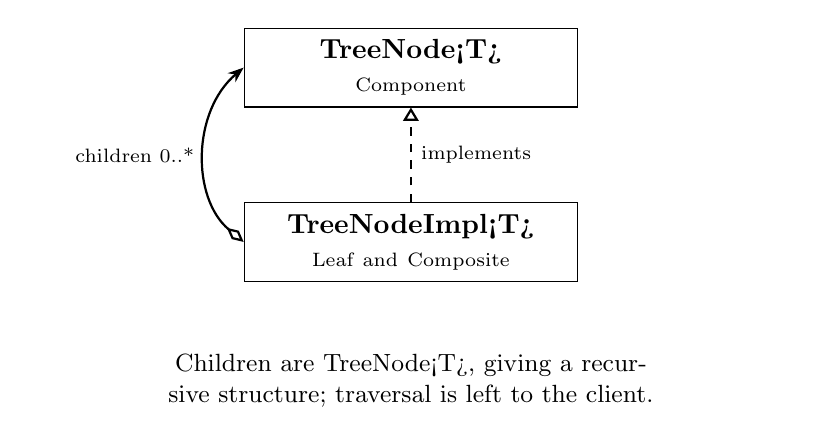
\begin{tikzpicture}[
  node distance=12mm and 15mm,
  cls/.style={draw,align=center,text width=40mm,minimum height=10mm},
  arr/.style={-{Stealth[length=2mm]},thick}
]
\node[cls] (component) {\textbf{TreeNode<T>}\\\scriptsize Component};
\node[cls,below=of component] (impl) {\textbf{TreeNodeImpl<T>}\\\scriptsize Leaf and Composite};
\draw[arr,dashed,-{Triangle[open]}] (impl)--node[right,font=\scriptsize]{implements}(component);
\draw[arr,{Diamond[open]}-{Stealth[length=2mm]}] (impl.west) to[bend left=50] node[left,font=\scriptsize]{children 0..*}(component.west);
\node[below=8mm of impl,align=center,text width=95mm,font=\small] {Children are \code{TreeNode<T>}, giving a recursive structure; traversal is left to the client.};
\end{tikzpicture}
\end{center}

\textbf{Verification and limitation.} Two Composite properties are present: part--whole recursion (children are themselves \code{TreeNode<T>}) and uniform treatment (child management is declared on the component interface, the GoF transparent form). There are no separate Leaf and Composite classes; "leaf" is a runtime state. \code{TreeNode} declares no recursive component operation, so the classification rests on structure and interface rather than recursive behavior. No concrete application/domain client using \code{TreeNode} or \code{TreeNodeImpl} was found, so the result is reported as a confirmed generic utility-level pattern instance, not evidence that a particular warehouse workflow uses Composite.

\subsection{Non-GoF mechanisms and rejected candidates}
Three further mechanisms were recorded separately from the GoF totals:

\begin{tabularx}{\linewidth}{@{}P{0.06\linewidth}P{0.27\linewidth}YP{0.17\linewidth}@{}}
\toprule
ID & Mechanism & Evidence & Status\\
\midrule
N01 & Asynchronous publish/subscribe & \code{EventPublisher.java:19-33}; \code{NonBlockingEventPublisherImpl.java:22-50} (\code{@Async publish} delegates to \code{dispatch}). & Confirmed\\
N02 & Spring application-event listener & \code{LocalServiceInitializer.java:27-33, 50-53} (\code{ApplicationListener<ContextRefreshedEvent>}). & Confirmed\\
N03 & Fire-after-transaction AOP advice & \code{FireAfterTransactionAspect.java:30-36, 52-66, 76-107}. The class is a plain \code{@Component}; no \code{@Aspect}, pointcut, XML \code{aop:} config or AspectJ dependency exists in the repository. & Partially confirmed (wiring not in scope)\\
\bottomrule
\end{tabularx}

\begin{tabularx}{\linewidth}{@{}lY@{}}
\toprule
Candidate & Reason for rejection\\
\midrule
Singleton & Spring \code{@Component} scope alone does not establish GoF Singleton. The candidate beans have public constructors and no static instance or accessor; they are single only because the container scopes them that way.\\
Proxy & Framework-generated proxies/AOP behavior is not counted as an application-level GoF Proxy, and no application class controls access to a separate subject through the same interface.\\
\bottomrule
\end{tabularx}
The rejected candidates and reasons are preserved in \code{Part1_Findings/data/rejected_candidates.csv}. These are scope-bounded rejections, not proof that the patterns occur nowhere in the larger ecosystem.

\section{Part 2 Evolution and refactoring}

The three changes are evaluated against their recorded acceptance criteria, commits, tests, and metrics. \textbf{Multiple-Warehouse Support} is an uncommitted modification to the existing OpenWMS Common Service worktrees. \textbf{Barcode-Based Picking} and \textbf{Automatic Stock Reordering} are separate reference applications, because the canonical Picking and Inventory modules were inaccessible. They must not be presented as upstream merged changes.

\subsection{\textbf{Multiple-Warehouse Support} --- Multiple warehouses}

\textbf{Change and acceptance criteria.} Introduce explicit warehouse identity so that locations with identical coordinate keys can exist in different warehouses without collision. A location belongs to one warehouse; location identity is the combination of warehouse and the existing five-part \code{LocationPK}. Coordinate uniqueness is warehouse-scoped, while PLC/ERP identifiers remain globally unique. \code{LocationGroup} remains a logical/hierarchical grouping rather than becoming a warehouse. Unqualified lookups that are ambiguous across warehouses must not silently choose one.

\textbf{Acceptance criteria and verification}

\begin{tabularx}{\linewidth}{@{}P{0.24\linewidth}P{0.22\linewidth}YP{0.14\linewidth}@{}}
\toprule
Criterion & Expected result & Verification evidence & Status\\
\midrule
Same coordinates in different warehouses & Both locations coexist, distinguished by warehouse. & \code{LocationTest.same_coordinates_in_different_warehouses_are_distinct_locations}; \code{LocationIT.shall_allow_same_coordinates_in_different_warehouses}. & Recorded as passed\\
Duplicate coordinates in one warehouse & Rejected by the warehouse-scoped uniqueness rule. & \code{UC_LOC_ID} constraint on (\code{C_WAREHOUSE}, \code{C_AREA}, \code{C_AISLE}, \code{C_X}, \code{C_Y}, \code{C_Z}); no test exercises the rejection. & Enforced by schema; not tested\\
Warehouse-qualified lookup & Resolves the location within that warehouse. & \code{LocationServiceImplIT.shall_allow_same_location_id_in_different_warehouses_and_find_by_warehouse}; \code{TransportUnitServiceImplIT.update_with_warehouse_code_selects_the_requested_warehouse_for_duplicate_coordinates}. & Recorded as passed\\
Ambiguous unqualified lookup & Not silently resolved. & \code{TransportUnitServiceImplIT.update_without_warehouse_code_rejects_an_ambiguous_coordinate}; \code{TransportUnitCommandHandlerIT.rejects_unqualified_creation_when_the_coordinate_is_ambiguous}. & Recorded as passed\\
PLC/ERP identifier uniqueness & Globally unique across warehouses. & \code{UC_LOC_PLC_CODE} and \code{UC_LOC_ERP_CODE}, unchanged from the baseline; no dedicated test. & Preserved by schema; not tested\\
LocationGroup semantics & Stays a logical hierarchy, not a warehouse. & Source/design review. & Preserved by design\\
Legacy constructor compatibility & Legacy \code{LocationMO} constructor still works. & \code{LocationMOTest.legacy_nine_argument_constructor_preserves_null_warehouse}. & Recorded as passed\\
Production data rollout & Existing locations assigned to warehouses before rollout. & No migration/backfill supplied. & Not completed\\
\bottomrule
\end{tabularx}
\textit{Status note:} the CH01 tests are identifiable by name in the published snapshot: 18 test methods were added (245 \code{@Test} annotations at the baseline, 263 after). The full list is in \code{report/part2_findings.pdf} and \code{Part2/CH01-multiple-warehouses/PROVENANCE.md}. The production rollout criterion is explicitly outstanding.

\textbf{Before and after.} The Common Service Library baseline is \code{a6566d7a90364f8cb0e82ec013720b644926dffe}; the Common Service baseline is \code{fc7edd4ffbe16de65d482b3a2d462d4d896b1998}. \textbf{Multiple-Warehouse Support} changes exist as uncommitted worktree changes in the two Common Service repositories; therefore there is no after commit ID. The re-audit re-derived the changed files by diffing the published snapshot against fresh upstream clones: 31 modified and 13 new files in the Library and 2 modified files in Common Service, exactly as recorded in \code{PROVENANCE.md}. No upstream commit or merge is claimed.

\textbf{Implementation.} The change adds a \code{Warehouse} entity (with controller, service, repository, mapper and API types) and a mandatory warehouse reference on \code{Location}, adds \code{C_WAREHOUSE} to the \code{UC_LOC_ID} uniqueness constraint, and adds warehouse-qualified behavior where needed. The existing coordinate key remains five-part. No automatic default warehouse or speculative data migration was added.

\textbf{Tests and recorded results.} The verification addendum records a direct Maven installation run for the Common Service Library with \code{-DforkCount=0}: 187 tests, zero failures/errors, and 7 skipped; the build reported \texttt{BUILD SUCCESS}, although Asciidoctor emitted errors in the build log. Common Service verification reported \texttt{BUILD SUCCESS}, 1 test, zero failures/errors/skips; Failsafe reported no integration tests. Because the fork configuration can reduce isolation and the documentation plugin emitted errors, these results should be interpreted with those caveats. See the dated addendum in \code{LLM_RECORDS/LLM_RECORDS.md}.

\textbf{Pattern effects.} No new GoF pattern was confirmed. \textbf{Multiple-Warehouse Support} extends the domain model and warehouse-qualified lookup behavior; the Part 1 Observer and Composite instance names remain unchanged. It is not evidence that the generic Composite utility became a domain-level warehouse hierarchy.

\textbf{Refactoring and behavior preservation.} The main structural change is replacing location-only identity assumptions with warehouse-qualified identity while preserving the existing coordinate key. The behavior-preservation cases are same coordinates in separate warehouses, ambiguity for unqualified lookups, warehouse-qualified transport-unit operations, and compatibility of the legacy \code{LocationMO} constructor; the named tests above cover them. A production rollout still requires an operator-supplied mapping/backfill for existing locations, because the new warehouse column is non-nullable.

\textbf{Before/after metrics.} No \textbf{Multiple-Warehouse Support} before/after LOC metrics were recorded. They are not estimated in this report. The after changes are not committed, so a stable after-commit measurement cannot be referenced.

\textbf{Limitations.} No Flyway/Liquibase migration or production backfill is included; ORM auto-update is not a substitute for a deployment-specific data migration plan. Existing production locations require an explicit warehouse assignment before rollout.

\subsection{\textbf{Barcode-Based Picking} --- Barcode-based picking}

\textbf{Change and acceptance criteria.} Add \code{POST /api/picking/barcode} to resolve a scanned barcode to stock and process a pick. A successful pick returns success; malformed/invalid requests return 400, unknown barcodes return 404, and unavailable or insufficient stock returns 409. The pre-existing item-ID route \code{POST /api/picking/item} remains separate.

\textbf{Acceptance criteria and verification}

\begin{tabularx}{\linewidth}{@{}P{0.24\linewidth}P{0.22\linewidth}YP{0.12\linewidth}@{}}
\toprule
Criterion & Expected result & Verification evidence (test methods) & Status\\
\midrule
Barcode endpoint, valid pick & Barcode resolves to stock and the pick succeeds. & \code{PickingControllerTest.post_valid_barcode_picks_stock_and_returns_result}; \code{PickingServiceTest.picks_stock_resolved_from_a_barcode_and_decreases_quantity}. & Passed\\
Invalid request & HTTP 400 for quantity below one. & \code{PickingControllerTest.post_zero_quantity_returns_bad_request}; \code{PickingServiceTest.rejects_zero_and_negative_quantities}. & Passed\\
Unknown barcode & HTTP 404, no stock created. & \code{PickingControllerTest.post_unknown_barcode_returns_not_found}; \code{BarcodeResolverTest.rejects_an_unknown_barcode_without_creating_stock}. & Passed\\
Unavailable/insufficient stock & HTTP 409. & \code{PickingControllerTest.post_unavailable_stock_returns_conflict}, \code{post_excessive_quantity_returns_conflict}; \code{PickingServiceTest.rejects_unavailable_stock}, \code{rejects_quantity_greater_than_available_stock}. & Passed\\
Existing item-ID route & Remains separate and available. & \code{PickingControllerTest.direct_item_id_endpoint_remains_separate_and_available}; \code{PickingServiceTest.direct_item_id_picking_remains_available_separately}. & Passed\\
\bottomrule
\end{tabularx}
\textit{Verification note:} the current source test total is 14 (6 controller, 2 resolver, 6 service), re-counted from the source in the re-audit. Stale ignored Surefire output for a missing integration-test source is excluded.

\textbf{Before and after.} Before commit: \code{5ca90cc12be1141be47cb6e6bdf3ca26efe636bd}. After commit: \code{0f0fbf0a3ca66c11f10cef127cbb2750a0ce53e8}. These commits belong to the original local project history, which was not copied into the team repository; only the after source tree is published there. The project is a standalone reference implementation, not a patch to the canonical OpenWMS Picking module.

\textbf{Implementation and tests.} Barcode resolution, pick-service behavior, and controller responses are separated into focused code and tests. Recorded \code{mvn.cmd -DforkCount=0 verify} completed with \textbf{BUILD SUCCESS}; 14/14 current source tests passed. The ignored generated \code{PickingControllerIT.xml/.txt} Surefire artifacts refer to a test source file that is absent; their reported six tests are stale and are explicitly excluded from the 14-test total.

\textbf{Pattern effects.} No new GoF pattern was confirmed. The MVC controller/service separation is continued; barcode lookup is a new use case, not sufficient by itself to claim Strategy, Adapter, or another GoF pattern.

\textbf{Refactoring.} The principal design improvement is separation of barcode resolution, pick validation/processing, and HTTP response mapping rather than embedding all behavior in one controller action. This is a reference implementation with in-memory demonstration storage, so the tests establish the behavior of this sample rather than production persistence or hardware integration.


\begin{tabularx}{\linewidth}{@{}lrr@{}}
\toprule
Metric & Before & After\\
\midrule
Production Java files & 7 & 14\\
Test Java files & 1 & 3\\
Total Java files & 8 & 17\\
Java LOC & 197 & 526\\
Test cases passed & 1 & 14\\
\bottomrule
\end{tabularx}
The after values were re-measured from the published source and match. The added LOC reflect added functionality and tests; more LOC is not itself evidence of better design.

\subsection{\textbf{Automatic Stock Reordering} --- Automatic stock-reorder rules}

\textbf{Change and acceptance criteria.} Reorder evaluation triggers when \code{availableQuantity <= reorderThreshold} and \code{availableQuantity < targetQuantity}. The requested quantity is \code{targetQuantity - availableQuantity}. Re-evaluation reuses an existing OPEN request. Completing a request replenishes stock and marks the request complete, allowing a later low-stock event to create a new request.

\textbf{Acceptance criteria and verification}

\begin{tabularx}{\linewidth}{@{}P{0.24\linewidth}P{0.22\linewidth}YP{0.12\linewidth}@{}}
\toprule
Criterion & Expected result & Verification evidence (test methods) & Status\\
\midrule
Threshold condition & Triggers only at or below threshold and below target. & \code{ReorderRuleTest.stock_above_threshold_does_not_require_reorder}, \code{stock_equal_to_threshold_requires_reorder_to_target}; \code{ReorderServiceTest.stock_above_threshold_does_not_create_a_request}. & Passed\\
Quantity calculation & Requested = target $-$ available. & \code{ReorderRuleTest.stock_below_threshold_calculates_quantity_to_target}; \code{ReorderServiceTest.stock_equal_to_threshold_creates_a_request_for_the_gap_to_target}, \code{stock_below_threshold_creates_a_request_for_the_gap_to_target}. & Passed\\
Rule validation & Negative threshold or target $\le$ threshold rejected. & \code{ReorderRuleTest.rejects_negative_threshold}, \code{rejects_target_that_is_not_greater_than_threshold}; \code{StockReorderControllerTest.invalid_rule_is_rejected}. & Passed\\
Open-request reuse & No duplicate while OPEN. & \code{ReorderServiceTest.repeated_evaluation_reuses_the_open_request}. & Passed\\
Completion and later reorder & Stock replenished; a later low-stock event creates a new request. & \code{ReorderServiceTest.automatic_reorder_after_consumption_and_completion_allow_a_future_request}, \code{completing_an_already_completed_request_is_rejected}; \code{StockReorderControllerTest.completing_request_replenishes_stock_and_allows_a_later_reorder}. & Passed\\
Persistence and distributed concurrency & State survives restart; distributed evaluation is safe. & Not implemented; storage is in memory and \code{evaluate}/\code{complete} are \code{synchronized} within one process. & Not satisfied\\
\bottomrule
\end{tabularx}
\textit{Verification note:} 19 test methods exist in the source (\code{ReorderRuleTest} 5, \code{ReorderServiceTest} 8, \code{StockReorderControllerTest} 4, \code{StockServiceTest} 2), matching the recorded 19/19. Further mappings for all eleven CH03 criteria are in \code{report/part2_findings.pdf}.

\textbf{Before and after.} Before commit: \code{e9ad4c171771f12865de763b7f99e909b2539c47}. After commit: \code{59b1b59ff6679d13d1c36781e2a76192bbb1a4c7}. As with Barcode-Based Picking, this history is not included in the team repository. This is a separate reference implementation, not a modification of the inaccessible canonical Inventory module.

\textbf{Implementation and tests.} The sample adds stock-rule and reorder-request operations, with endpoints for reading/consuming stock, managing rules, evaluating reorders (204 when no reorder is needed), listing and retrieving requests, and completing requests. Recorded \code{mvn.cmd -DforkCount=0 verify} completed with \texttt{BUILD SUCCESS}; 19/19 tests passed.

\textbf{Pattern effects.} No new GoF pattern was confirmed. The rule predicate does not by itself establish Strategy because the implementation does not demonstrate a family of interchangeable algorithms selected through a common strategy abstraction. Existing MVC and repository-style separation is extended.

\textbf{Refactoring and limitations.} The implementation separates stock, rule, and request responsibilities and makes repeated evaluation idempotent while a request remains OPEN. Storage is in memory, not durable; synchronization is only within the application process. It is not production-ready for concurrent distributed deployments without persistence and concurrency control.


\begin{tabularx}{\linewidth}{@{}lrr@{}}
\toprule
Metric & Before & After\\
\midrule
Production Java files & 6 & 24\\
Test Java files & 1 & 4\\
Total Java files & 7 & 28\\
Java LOC & 169 & 978\\
Test cases passed & 2 & 19\\
\bottomrule
\end{tabularx}
The after values were re-measured from the published source and match.

\subsection{Updated pattern counts and interpretation}
Across the recorded changes, the confirmed GoF inventory remains Observer and Composite: 2 distinct types and 2 instances in the Part 1 baseline. \textbf{Barcode-Based Picking} and \textbf{Automatic Stock Reordering} explicitly introduce no new confirmed GoF instance. \textbf{Multiple-Warehouse Support} changes warehouse domain identity and lookup behavior but does not establish a new GoF collaboration. The confirmed baseline participant count remains the Part 1 count; no new GoF participants are added to that inventory by these evolution scenarios. The Part 1 inventory is intentionally not inflated by ordinary controller, service, entity, or repository classes.

\begin{tabularx}{\linewidth}{
    @{}
    >{\raggedright\arraybackslash}p{0.22\linewidth}
    *{4}{>{\centering\arraybackslash}p{0.095\linewidth}}
    >{\raggedright\arraybackslash}X
    @{}
}
\toprule
Snapshot / change & Types & Instances & Concrete classes & Rejected candidates & Notes\\
\midrule
Part 1 baseline
& 2 & 2 & 2 & 2
& Observer and generic Composite confirmed.\\

After \textbf{Multiple-Warehouse Support}
& 2 & 2 & 2 & 2
& No new GoF pattern confirmed; changes remain uncommitted.\\

After \textbf{Barcode-Based Picking}
& 2 & 2 & 2 & 2
& Separate reference implementation; no new GoF pattern.\\

After \textbf{Automatic Stock Reordering}
& 2 & 2 & 2 & 2
& Separate reference implementation; no new GoF pattern.\\
\bottomrule
\end{tabularx}

The counts describe the frozen Part 1 inventory carried forward for cross-part consistency, not an exhaustive new pattern scan of each reference project. Changes are valuable because they address the requirements and clarify responsibilities; raw LOC increases do not prove design quality.

\section{Part 3 Cross-language comparison}

\subsection{Selected instances and common specifications}
The selected patterns are the source-verified Observer and Composite concepts from Part 1. The four-language implementations are independent, small reference implementations used to compare expression of the same concepts; they do not modify or claim to reproduce the internal OpenWMS implementation.

\textbf{Observer specification.} Support subscribe, unsubscribe, and publish. With three observers registered, publish \code{STOCK_LOW}; unsubscribe observer 2; publish \code{STOCK_REPLENISHED}. The second publication must reach observers 1 and 3, but not observer 2.

\textbf{Composite specification.} Represent a hierarchy \code{Warehouse > Zone-A > A-01/A-02} and \code{Warehouse > Zone-B > B-01}. Nodes share a common interface for name, child addition/removal, child retrieval, and recursive preorder traversal. Unlike the OpenWMS \code{TreeNode}, these implementations use separate \code{Container} and \code{Leaf} classes and include a recursive \code{traverse} operation on the component.

\subsection{Implementations and actual results}
The source and executable test harnesses are grouped under \code{Part3-cross-language/observer/} and \code{Part3-cross-language/composite/}, with Java, Python, JavaScript, and C++ subdirectories. Toolchain versions are listed in the environment section and detailed in \code{Part3-cross-language/PART3_EVIDENCE.md}. All eight pattern/language combinations passed: Observer 3/3 and Composite 4/4 in each language, for 28/28 checks overall. The re-audit re-ran all eight harnesses on a second machine and toolchain and again obtained 28/28. Per-harness console log files were not retained in the published evidence tree; the recorded commands/results should not be misrepresented as attached raw logs.

\subsection{Static metrics}
The following LOC totals include implementation and test code. Maximum cyclomatic complexity is the recorded Lizard 1.24.1 result; complexity-parser semantics are tool-dependent. All values were recomputed in the re-audit and match.

\begin{tabularx}{\linewidth}{@{}llrrrrr@{}}
\toprule
Pattern & Language & Impl.\ LOC & Test LOC & Total LOC & Max CCN & Checks passed\\
\midrule
Observer & Java & 65 & 70 & 135 & 2 & 3/3\\
Observer & Python & 52 & 37 & 89 & 3 & 3/3\\
Observer & JavaScript & 54 & 43 & 97 & 2 & 3/3\\
Observer & C++ & 55 & 61 & 116 & 2 & 3/3\\
Composite & Java & 89 & 63 & 152 & 2 & 4/4\\
Composite & Python & 71 & 48 & 119 & 2 & 4/4\\
Composite & JavaScript & 81 & 47 & 128 & 2 & 4/4\\
Composite & C++ & 85 & 62 & 147 & 2 & 4/4\\
\bottomrule
\end{tabularx}

The machine-readable values are in \code{Part3-cross-language/metrics/cross_language.csv} and \code{pattern_metrics.csv}. The recorded timing protocol used one warm-up and 30 timed process invocations; Java/C++ compilation was excluded. The workload is very small and process startup dominates, so the timing values do not support a language-performance ranking. The CSV is the source of record for any timing values; no timing value is inferred in this summary.

\subsection{Comparison and technology discussion}
Observer maps naturally to interfaces and listener collections in Java, ABC-based contracts and object lists in Python, base classes and arrays in JavaScript, and pure virtual classes with non-owning pointers in C++. The important design property is the ability to register and remove independent consumers without making the publisher encode each consumer's behavior. Composite benefits from a shared component abstraction and recursive composition: clients can traverse a container and its descendants uniformly. Java expresses the abstraction through interfaces/classes; Python and JavaScript can express the same contract with less ceremony; C++ expresses it through classes and explicit ownership (\code{std::shared_ptr} children). These are qualitative observations from the small examples, not general performance claims.

The source artifacts, metrics, and exact commands are documented in \code{PART3_EVIDENCE.md}.

\section{LLM records and human verification}

The evidence record is \code{LLM_RECORDS/LLM_RECORDS.md}, with \code{Part3-cross-language/metrics/llm_records.csv} as its machine-readable index. Eight LLM-related records are present, including the 11 October re-audit (AUDIT-01). Four exact prompts are available; four records have historical prompt/model/access-tier metadata that could not be recovered. The report preserves that limitation rather than inventing model names, dates, or outputs.

\begin{tabularx}{\linewidth}{@{}lYY@{}}
\toprule
Area & Verification evidence & Remaining limitation\\
\midrule
Part 1 & Source-based mappings re-checked line by line against the baseline; copied sources byte-identical; rejected candidates, counts, and notes. & Library scope: no concrete \code{EventListener} and no \code{TreeNode} client; N03 AOP wiring not in the repository.\\
\textbf{Multiple-Warehouse Support} & Dated verification addendum; changed-file list re-derived against upstream; 18 named CH01 test methods. & Changes uncommitted; no after commit ID or LOC metrics; migration/backfill absent; duplicate-coordinate rejection not tested; Asciidoctor errors noted.\\
\textbf{Barcode-Based Picking} & Source tests by name, acceptance criteria, commit pair, before/after metrics; after metrics re-measured. & Commit history not in the team repository; stale Surefire output excluded; no production storage/hardware claim.\\
\textbf{Automatic Stock Reordering} & Source tests by name, acceptance criteria, commit pair, before/after metrics; after metrics re-measured. & Commit history not in the team repository; in-memory state and single-process synchronization only.\\
Part 3 & Eight implementations, 28/28 checks (re-run), CSV metrics (recomputed), documented timing protocol. & Per-harness raw console logs were not retained; timing not re-measured.\\
\bottomrule
\end{tabularx}

Generated code was treated as a candidate contribution and checked against the source, tests, and documented acceptance criteria. LLM-generated statements were not accepted as evidence without verification. Maven builds could not be re-run in the re-audit, so their totals remain the team's recorded runs. Missing historical details remain marked as unavailable.

\section{Findings, contributions and references}

\subsection{Findings}
\begin{enumerate}[leftmargin=*,nosep]
\item The OpenWMS CORE baseline supports two confirmed GoF pattern instances: an Observer event-dispatching collaboration, with the Subject split into registration and notification interfaces, and a transparent, single-class Composite tree utility.
\item Both instances are confirmed at library level: the inspected repository contains no concrete \code{EventListener} and no client of \code{TreeNode}.
\item The OpenWMS Observer matches subscribers by exact event class and notifies them synchronously; asynchrony comes from the separate publisher (N01).
\item The OpenWMS Composite has no recursive component operation; it is a Composite by structure and interface rather than by recursive behavior.
\item \textbf{Multiple-Warehouse Support} models warehouse-scoped location identity and passes its recorded verification, but the work remains uncommitted, duplicate-coordinate rejection is enforced by schema without a test, and production rollout needs a deployment-specific mapping/backfill plan.
\item \textbf{Barcode-Based Picking} demonstrates barcode-driven picking behavior with 14/14 tests in a standalone reference project; it is not a change to the canonical Picking module.
\item \textbf{Automatic Stock Reordering} demonstrates threshold/target-based automatic reorder behavior with 19/19 tests in a standalone reference project; its in-memory state and single-process synchronization are not production persistence/concurrency controls.
\item Part 3 demonstrates consistent Observer and Composite behavior in Java, Python, JavaScript, and C++, with 28/28 checks reproduced on two toolchains and recorded static metrics. Its tiny timing workload does not justify performance conclusions.
\item The evidence shows requirement coverage and separation of responsibilities, but neither LOC growth nor passing tests alone establishes that a design is universally better.
\end{enumerate}

\subsection{Team contributions}
The final contribution statements must be reviewed and confirmed by all team members. The current record intentionally does not infer individual work allocation from the roster alone.

\begin{tabularx}{\linewidth}{@{}lllY@{}}
\toprule
Roll number & Name & Batch & Contribution\\
\midrule
AM.SC.U4CSE23215 & D Aditya Kiran & CSE C & To be confirmed by the team against actual work and commits.\\
AM.SC.U4CSE23235 & Mithun Krishna & CSE C & To be confirmed by the team against actual work and commits.\\
AM.SC.U4CSE23248 & Sai Kishen K M & CSE C & To be confirmed by the team against actual work and commits.\\
AM.SC.U4CSE23359 & Sivadev Smijith & CSE D & To be confirmed by the team against actual work and commits.\\
\bottomrule
\end{tabularx}

\subsection{References and evidence artifacts}
\begin{enumerate}[leftmargin=*,nosep]
\item OpenWMS CORE repository: \url{https://github.com/openwms/org.openwms}, baseline \code{9d263bf65ec75301e0302539ae7bf581412742b8}; source of the Part 1 classes and of the README statements on architecture and module accessibility.
\item OpenWMS Common Service Library: \url{https://github.com/openwms/org.openwms.common.service.lib}, baseline \code{a6566d7a90364f8cb0e82ec013720b644926dffe}.
\item OpenWMS Common Service: \url{https://github.com/openwms/org.openwms.common.service}, baseline \code{fc7edd4ffbe16de65d482b3a2d462d4d896b1998}.
\item Part 1 findings and counts: \code{Part1_Findings/Part1_Findings.md}; \code{Part1_Findings/data/patterns.csv}; \code{Part1_Findings/data/pattern_counts.csv}; \code{Part1_Findings/data/rejected_candidates.csv}; \code{Part1_Findings/evidence/verification_notes.md}.
\item Part 1 diagrams: \code{observer_uml.puml}, \code{composite_uml.puml}, and \code{architecture_scope.puml}, with rendered PNGs, in \code{Part1_Findings/diagrams/}.
\item \textbf{Multiple-Warehouse Support} provenance and verification: \code{Part2/CH01-multiple-warehouses/PROVENANCE.md}; \code{LLM_RECORDS/LLM_RECORDS.md}, including the dated verification addendum.
\item \textbf{Barcode-Based Picking} evidence and source: \code{Part2/CH02-barcode-picking/CH02_EVIDENCE.md}; before commit \code{5ca90cc12be1141be47cb6e6bdf3ca26efe636bd}; after commit \code{0f0fbf0a3ca66c11f10cef127cbb2750a0ce53e8}.
\item \textbf{Automatic Stock Reordering} evidence and source: \code{Part2/CH03-stock-reorder/CH03_EVIDENCE.md}; before commit \code{e9ad4c171771f12865de763b7f99e909b2539c47}; after commit \code{59b1b59ff6679d13d1c36781e2a76192bbb1a4c7}.
\item Part 3 implementations, metrics, and evidence: \code{Part3-cross-language/PART3_EVIDENCE.md}; \code{Part3-cross-language/metrics/cross_language.csv}; \code{Part3-cross-language/metrics/pattern_metrics.csv}; \code{Part3-cross-language/metrics/llm_records.csv}.
\item Complexity tool: Lizard 1.24.1, recorded in the Part 3 evidence. Compiler/runtime versions are listed in the same evidence.
\item E.~Gamma, R.~Helm, R.~Johnson and J.~Vlissides, \textit{Design Patterns: Elements of Reusable Object-Oriented Software}, Addison-Wesley, 1994 (Observer, Composite, Singleton, Proxy).
\end{enumerate}

\section{Team folder and datasets}
The team working repository keeps the report, raw inventories, change-case evidence, tests, and cross-language metrics traceable. Its current organization is:
\begin{verbatim}
Team_B9_DP/
  README.md
  report/
    main.tex, main.pdf
    part1_findings.tex/.pdf, part2_findings.tex/.pdf, part3_findings.tex/.pdf
  Team_B9_Findings/
    README.md
    COPY_MANIFEST.md
    LLM_RECORDS/LLM_RECORDS.md
    Part1_Findings/
      Part1_Findings.md
      data/  diagrams/  evidence/
    Part2/
      CH01-multiple-warehouses/
      CH02-barcode-picking/
      CH03-stock-reorder/
    Part3-cross-language/
      observer/  composite/  metrics/
      PART3_EVIDENCE.md
\end{verbatim}
The CH02 and CH03 Git histories (and therefore their before commits) and the CH01 upstream worktrees are not part of this repository; upstream OpenWMS source is included only as the evidence excerpts and snapshots described in \code{COPY_MANIFEST.md}, with Apache 2.0 notices preserved. The repository screenshot required by the assignment should be captured from the final published submission repository.

\end{document}
